\section{intro v1}
%Powered by large language models (LLMs), role-playing agents support a wide range of interactive applications, from interactive NPCs in immersive gaming to virtual characters in narrative experiences. Unlike traditional instruction-following assistants, role-playing agents in immersive environments necessitate the maintenance of a coherent persona throughout extended, multi-turn conversations. While current LLMs excel at generating fluent isolated responses, the essence of role-playing lies not in single turns, but in the coherence of the entire session. How to faithfully evaluate the quality of such sustained interactions, however, remains an open challenge.

%Prevalent evaluation approaches for role-playing agents, such as InCharacter \cite{}, CharacterBench \cite{}, and CharacterEval \cite{}, define diverse assessment dimensions (e.g., knowledge, personality, style), yet share a common scoring mechanism that judges quality based on a single model response given a persona description and dialogue history. CharacterBench \cite{} acknowledges that certain dimensions, termed ``sparse'' attributes such as memory consistency and behavior consistency, are difficult to observe in a single exchange. Consequently, it introduces targeted queries designed to probe these traits.  However, this approach evaluates each response in isolation, failing to detect patterns that emerge across turns, such as repeated phrasing, or to identify a character whose consistency gradually erodes.

%This paradigm mismatch has concrete consequences, as illustrated in Figure~\ref{fig:teaser}. Consider a model that generates a vivid, expressive response in a single turn---one that scores highly on human-likeness. Yet across a full conversation, the same model may fall into recycling the same phrasing templates turn after turn—a failure mode that response-level evaluation cannot detect. The same problem arises with interactivity: a model may seem appropriately proactive when it poses a question in one turn, yet when this behavior persists across the session, it becomes a repetitive questioning pattern that disrupts conversational flow. In both cases, the high-scoring isolated response actively misleads the evaluation—single-turn metrics reward local quality while remaining blind to session-level failures that matter most in practice.

%To address this discrepancy, evaluation must shift from individual responses to complete dialogue sessions. We introduce a \textbf{session-level evaluation framework} that assesses role-playing performance across four dimensions: Human-likeness, Role Consistency, Context Consistency, and Interactive Ability. These dimensions capture cumulative conversational patterns that single-turn metrics miss. The framework first generates evaluation sessions by pairing the model with a human user or a dialogue simulator under a specific persona and scenario. An LLM-as-a-Judge then scores the complete session. Because the judge evaluates the entire exchange, it can penalize repetitive or drifting behaviors that look fine in isolation. As Section~\ref{sec:experiments} shows, this session-level scoring aligns much more closely with human judgments of interaction quality.

%This turn-level myopia also affects how these models are trained. Standard DPO~\cite{PLACEHOLDER_dpo} and its variants construct preference pairs at the turn level. Because they optimize responses in isolation, they struggle to enforce consistent character behavior throughout a long conversation. We therefore propose \textbf{Session-level DPO (S-DPO)} to align models over complete sessions. Instead of comparing single responses, S-DPO constructs preference pairs $(\mathcal{S}_w, \mathcal{S}_l)$ over full dialogues. The reward signal comes from the cumulative log-likelihood ratio across the session, allowing the model to learn behavioral patterns that turn-level optimization misses. Under our evaluation framework, S-DPO consistently outperforms both the base model and turn-level DPO baselines in automated scoring and win-rate assessments.


\section{* intro v2}

With the rapid development of Large Language Models and intelligent agents, role-play agents have attracted widespread interest and have been deployed on a massive scale in scenarios such as emotional companionship and  gaming interactions \cite{tseng-etal-2024-two, chen2024persona}. Role-playing agents foster a more natural and immersive interaction experience while strictly conforming to designated personas, thereby significantly boosting user satisfaction and emotional resonance. Consequently, accurately evaluating and iteratively improving the conversational capabilities of these generative models has emerged as a crucial research topic \cite{wang-etal-2024-rolellm, lu-etal-2024-large}.

A substantial body of work has been dedicated to evaluating the capabilities of role-play models. Specifically, existing methodologies often employ \textbf{LLMs} as judges to assess generated responses based on predefined criteria regarding persona and linguistic style. For instance, InCharacter\cite{wang-etal-2024-rolellm} evaluates the persona consistency of role-play models by prompting them to act as psychotherapists. Taking a step further, CharacterEval \cite{wang-etal-2024-rolellm} introduced a multi-dimensional evaluation metric incorporating knowledge boundaries and linguistic styles. However, these approaches primarily evaluate the quality of a single-turn response given a static persona and pre-defined dialogue context. In reality, role-playing is a continuous, long-term process heavily dependent on dynamic user interactions. Such static, short-term modeling fails to accurately capture the true user experience in real-world conversational scenarios.

As illustrated in Fig. 1, when a user initially expresses negative emotions, the model may generate a superficially appropriate and comforting response. Traditional turn-level metrics often interpret such behavior as strong emotional empathy (View 1). However, as the dialogue proceeds across multiple turns, the model’s responses gradually degenerate into mechanical repetition and shallow comfort. In summary, evaluation paradigms limited to single-turn responses are inherently unable to capture higher-level dimensions such as interaction depth and emotional progression, which are critical for assessing role-play agents.

\begin{figure*}[t]
  \centering
  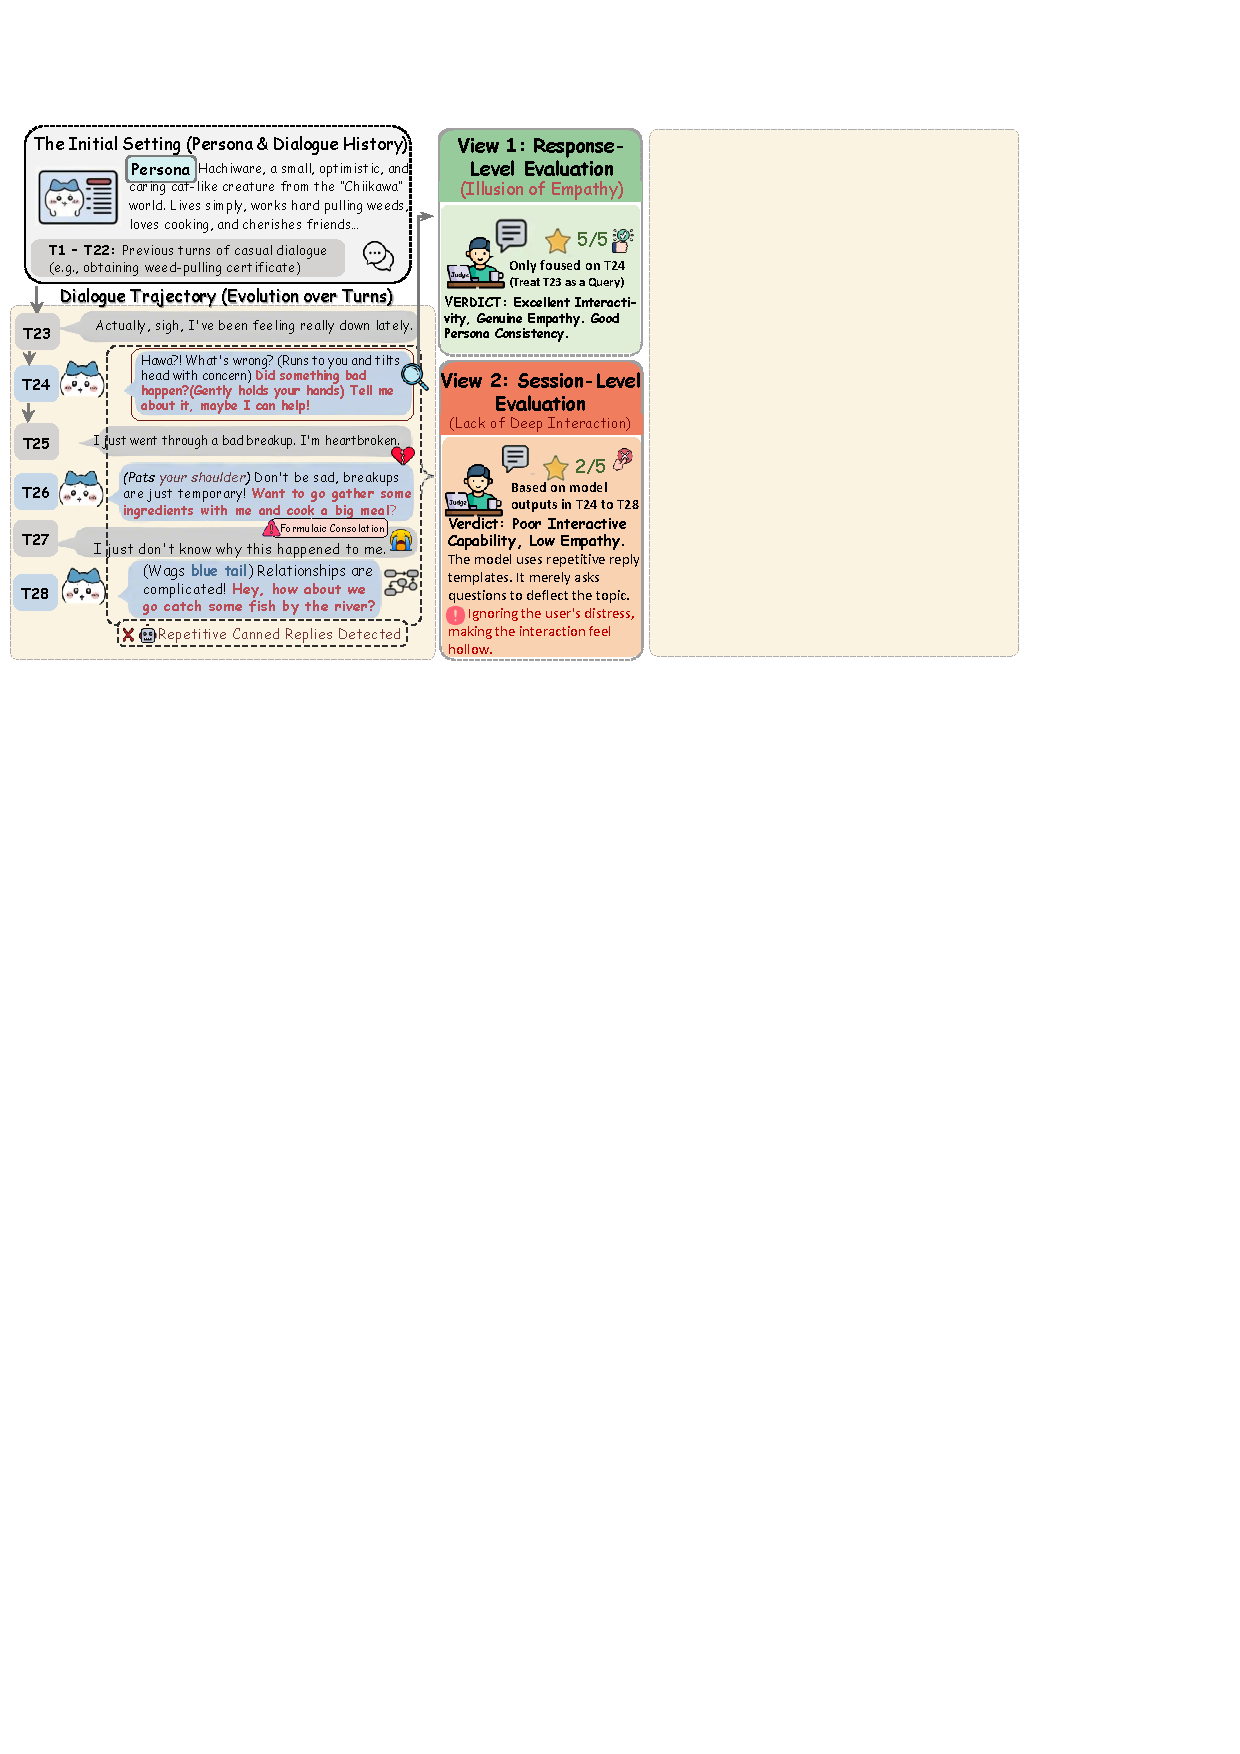
\includegraphics[
    width=\textwidth,
    trim=0 18.5cm 3.5cm 2cm,
    clip
  ]{latex/Image/intro2.pdf}
  \caption{A figure with a caption that runs for more than one line.
    Example image is usually available through the \texttt{mwe} package
    without even mentioning it in the preamble.}
  \label{fig:experiments}
\end{figure*}

Recently, several studies have recognized the limitations of previous evaluation metrics. CharacterBench \cite{wang-etal-2024-rolellm} was the first to note that certain capabilities of role-play models are sparse and cannot be adequately reflected by a single arbitrary response, thus it designed fixed contexts to test specific capabilities. RMTBench \cite{xiang-etal-2025-rmtbench} further designed a semi-dynamic multi-turn evaluation set based on offline real user interactions. Nevertheless, these methods still fundamentally rely on static contexts—essentially conducting pseudo-multi-turn evaluations, where the final score depends solely on the last generated response, failing to reflect the dynamic evolution of dialogue guidance and emotional transitions. Conversely, CharacterArena \cite{ye-etal-2025-cpo} introduced a dynamic context approach, evaluating the superiority of generated trajectories at the session level via pairwise comparisons. However, as a comprehensive ranking system, it primarily provides relative preference signals, struggling to offer independent, fine-grained diagnostic results across specific dimensions for a single session. Furthermore, it does not systematically answer which session-level dimensions are most critical in role-playing, thereby limiting the interpretability of the results and offering little actionable guidance for model iteration.

To address these aforementioned challenges, we propose DYNSESS-EVAL, a dynamic, session-level evaluation framework specifically tailored for role-play agents. Distinct from prior works, we innovatively adopt a multi-agent interaction paradigm, where dynamic dialogue sessions are entirely generated through autonomous interactions between a User-agent and a Character-agent—this design effectively captures the model’s long-term interactive capabilities in a realistic scenario. Furthermore, we identify and formalize four critical session-level dimensions that are pivotal to the performance of role-play agents, namely Human-likeness, Character Consistency, Contextual Coherence, and Proactiveness, and correspondingly construct dedicated evaluation datasets and standardized methodologies. Experimental results demonstrate that, compared with human expert annotations, our dynamic session-level evaluation approach achieves significantly better alignment, outperforming all existing baselines by a substantial margin.

Moreover, our evaluations demonstrate that current role-play agents exhibit poor performance on these long-term interaction metrics. Early alignment approaches (e.g., standard Supervised Fine-Tuning (SFT) or Reinforcement Learning from Human Feedback (RLHF)) typically focus on optimizing the model’s single-turn response quality, while neglecting the modeling of long-term dynamic interactions. For instance, standard Generative Reward Policy Optimization (GRPO) or Direct Preference Optimization (DPO) methods rely on step-wise preference signals, which are insufficient to optimize the cumulative conversational experience over extended interactions. To address this limitation, we propose a Session-level Reinforcement Learning (SRL) approach. During the candidate generation phase, SRL leverages multi-agent interaction simulations to generate long-context rollouts. By introducing session-level reward signals, we directly optimize the role-play agent for long-term conversational efficacy. Experimental results validate that our proposed SRL method significantly improves the performance of role-play agents, achieving state-of-the-art (SOTA) results on the evaluated metrics.


Overall, our contributions are three-fold:
\begin{itemize}
\item We propose a dynamic session-level evaluation framework that significantly improves the assessment of role-play agents across four key dimensions, thereby bridging the gap between automatic evaluation and human expert annotations.
\item We introduce a Session-level Reinforcement Learning (SRL) method tailored specifically for persona-driven dialogue scenarios, which substantially enhances the long-term conversational capabilities of role-play agents.
\item Our proposed evaluation framework, DYNSESSEVAL, achieves superior performance in multi-turn conversational assessments, and the role-play agents optimized via our SRL method attain state-of-the-art (SOTA) capabilities.
\end{itemize}

\section{method v1}



\begin{figure*}[t]
  \includegraphics[width=\textwidth, trim = 0 3cm 0 0, clip]{latex/Image/methodv2.png}

  \caption{A figure with a caption that runs for more than one line.
    Example image is usually available through the \texttt{mwe} package
    without even mentioning it in the preamble.}
  \label{fig:experiments}
\end{figure*}

In this section, we introduce our framework for evaluating and optimizing role-playing agents in long-term interactions.  including \textbf{DynSessEval} for dynamic session-level evaluation (Section 3.1) and \textbf{SRL} for multi-turn trajectory optimization (Section 3.2).

% In this section, we present our comprehensive framework for evaluating and optimizing role-playing agents in continuous, long-term interactions. First, we introduce \textbf{DynSessEval}, a dynamic session-level evaluation framework driven by a multi-agent interaction mechanism (Section 3.1). Subsequently, to address the shortcomings of existing models in long-term engagement, we propose \textbf{SRL} (Session-level Reinforcement Learning), a novel training paradigm that optimizes role-playing agents over multi-turn trajectories rather than single-turn responses (Section 3.2).

\subsection{ \textsc{DynSessEval}: Dynamic Session-Level Evaluation Framework}

%Unlike traditional static evaluations that assess single-turn responses given fixed historical contexts, \textsc{DynSessEval} constructs fully dynamic, multi-turn dialogue sessions to evaluate agent performance comprehensively.

\textbf{Multi-Agent Interaction}. To simulate realistic and continuous user--character interactions, we employ a multi-agent framework consisting of a User Agent and a Character Agent. Given a target character persona $P_C$, we instantiate the User Agent with a persona $P_U$ generated by an LLM conditioned on $P_C$ and a prompting template $I$:
\begin{equation}
P_U = \mathcal{G}(P_C, I)
\end{equation}
where $\mathcal{G}(\cdot)$ denotes the persona generation function.
% To simulate realistic and continuous user–character interactions, we employ a multi-agent framework consisting of a User Agent and a Character Agent. Given a target character persona $P_C$, we first design a human prior–based prompt $I$ for persona generation, then initialize the User Agent to behave as a human interlocutor.To ensure the diversity and contextual relevance of the simulated user, we dynamically generate the user persona $P_U$ from the character persona and the designed prompt:
% \begin{equation}
% P_U = \mathcal{G}(P_C, I)
% \end{equation}
% where \( \mathcal{G}(\cdot) \) denotes the persona generation function implemented by an LLM.



% where  \( \mathcal{G} \) 
%  denotes a large language model (LLM) used as the persona generator.

% During the simulation, at the $t$-th turn, the User Agent generates a query $u_t$ based on its persona $P_U$ and the current dialogue history $H_{t-1} = \{(u_1, c_1), \dots, (u_{t-1}, c_{t-1})\}$. The Character Agent then produces a response $c_t$ conditioned on $P_C$ and $H_{t-1} \cup \{u_t\}$. This process is repeated iteratively to generate a full dynamic session:
% %少了一部分persoina
% \begin{equation}
% \begin{split}
%     u_t &\sim \pi_{\text{user}}(\cdot \mid P_U, H_{t-1}) \\
%     c_t &\sim \pi_{\theta}(\cdot \mid P_C, H_{t-1}, u_t)
% \end{split}
% \end{equation}
% where $\pi_{\theta}$ denotes the role-playing model being evaluated. The resulting trajectory $\tau = \{(u_1, c_1), \dots, (u_T, c_T)\}$ effectively captures the long-term interaction dynamics.

During the simulation, at turn $t$, the User Agent generates an query $u_t$ based on its persona $P_U$ and the dialogue history $H_{t-1} = \{(u_1, c_1), \dots, (u_{t-1}, c_{t-1})\}$. The Character Agent, i.e., the model under evaluation, then produces a response $c_t$ conditioned on $P_C$, $H_{t-1}$, and $u_t$. Formally,
\begin{equation}
\begin{split}
    u_t &\sim \pi_{\text{user}}(\cdot \mid P_U, H_{t-1}) \\
    c_t &\sim \pi_{\theta}(\cdot \mid P_C, H_{t-1}, u_t)
\end{split}
\end{equation}
Repeating this process for $T$ turns yields a session trajectory $\tau = \{(u_1, c_1), \dots, (u_T, c_T)\}$, which serves as the basis for evaluating long-term interaction dynamics.


\noindent \textbf{Session-Level Evaluation Dimensions.}
To accurately diagnose the quality of the generated session $\tau$, we define four critical session-level dimensions:
\begin{itemize}[leftmargin=*]
\item \textbf{Interactive Ability} ($D_{Pro}$): Examines the agent's ability to actively sustain and advance the conversation by introducing relevant topics, follow-up questions, or developments, rather than merely reacting passively to user inputs.

\item \textbf{Human-likeness} ($D_{HL}$): Evaluates whether the character exhibits natural and human-like behavior across multiple turns, including smooth emotional progression and avoidance of mechanical, repetitive, or formulaic responses.

\item \textbf{Character Consistency} ($D_{CC}$): Measures the degree to which the agent adheres to its predefined persona $P_C$ (e.g., tone, speaking style, background knowledge, and behavioral traits) throughout the entire session.

\item \textbf{Contextual Coherence} ($D_{Coh}$): Assesses the logical continuity of the multi-turn interaction, including whether the agent correctly maintains, recalls, and references prior conversational context across turns.
\end{itemize}
% Human-likeness ($D_{HL}$): Evaluates whether the character exhibits natural, human-like emotional progression and avoids mechanical, repetitive comfort over multiple turns.
% Character Consistency ($D_{CC}$): Measures the degree to which the agent adheres to its predefined persona $P_C$ (e.g., tone, catchphrases, and background knowledge) throughout the entire session.
% Contextual Coherence ($D_{Coh}$): Assesses the logical flow and transition of topics across the multi-turn session, ensuring the agent correctly remembers and references earlier parts of the conversation.
% Proactiveness ($D_{Pro}$): Examines the agent's ability to drive the conversation forward, introduce relevant topics, and actively engage the user rather than passively answering questions.

To quantify these dimensions, we adopt the LLM-as-a-Judge paradigm. We design customized evaluation rubrics $R_d$ for each dimension $d \in \{D_{HL}, D_{CC}, D_{Coh}, D_{Pro}\}$. A powerful LLM acts as the evaluator $J$, taking the entire session $\tau$, the persona $P_C$, and the rubric $R_d$ as input to produce a scalar score $s_d$ and a natural language justification.
%把公式展开成复杂形式，人设，对话历史
\begin{equation}
    s_d = J(\tau, P_C, R_d)
\end{equation}

\noindent \textbf{Evaluation Procedure}
Our evaluation pipeline is designed to be highly automated and scalable. To thoroughly test the agent's capabilities, we construct two distinct dataset settings:
- **Non-history Setting:** The interaction starts from scratch given only the persona $P_C$ and a greeting. This tests the agent's ability to establish character identity and build rapport from the ground up.
- **With-history Setting:** The interaction is initialized with a pre-existing dialogue context $H_{init}$. This evaluates the agent's capacity for context integration and long-term memory retrieval.

The overall procedure operates as follows: Given $P_C$ and an optional $H_{init}$, the multi-agent simulation continuously interacts to generate a full dynamic session $\tau$ of length $T$. Finally, the LLM evaluator $J$ is applied to $\tau$ across all four dimensions, yielding a comprehensive session-level performance profile for the model.


\subsection{\textsc{SRL}: Session-Level Reinforcement Learning}

Observations from our \textsc{DynSessEval} framework indicate that models optimized solely via Supervised Fine-Tuning (SFT) or traditional Reinforcement Learning (RL) struggle with long-term metrics. To bridge this gap, we introduce Session-Level Reinforcement Learning (\textsc{SRL}).

 \textbf{Turn-level RL.}
Previous RL approaches for LLMs (e.g., RLHF) primarily focus on single-turn optimization. Given a static context $x$ (which may include history), the model $\pi_\theta$ generates a single response $y$. A reward model $r_\phi$ assigns a scalar reward $R = r_\phi(x, y)$. The objective is to maximize the expected reward while penalizing deviation from a reference policy $\pi_{\text{ref}}$:

\begin{align}
    \max_{\theta} \mathbb{E}_{x \sim \mathcal{D}, y \sim \pi_\theta(\cdot|x)} \left[ 
    &r_\phi(x, y) - \beta \mathbb{D}_{\text{KL}} \right. \notag \\
    &\left. (\pi_\theta(\cdot|x) \| \pi_{\text{ref}}(\cdot|x)) \right]
\end{align}

Because the rollout and reward are computed on a per-response basis, the model is disincentivized from performing strategic, multi-turn dialogue planning (e.g., gradually building emotional resonance).

\textbf{Multi-Agent Rollout and Session-Level Reward.}
To optimize the long-term interaction quality, \textbf{SRL} extends the optimization horizon to the entire dialogue session. During the training phase, we leverage the multi-agent simulation introduced in Section 3.1.1 to generate multi-turn rollouts. 

For a given persona $P_C$, the User Agent $\pi_{\text{user}}$ and the active policy $\pi_\theta$ interact for $T$ turns, generating a trajectory $\tau = (u_1, c_1, \dots, u_T, c_T)$. Instead of applying a reward to each $c_t$ individually, we utilize a Session-level Reward Model $R_{\Phi}$ that evaluates the holistic quality of the entire trajectory based on our defined dimensions (Human-likeness, Consistency, Coherence, Proactiveness):
\begin{equation}
    R_{\text{session}} = R_{\Phi}(\tau, P_C)
\end{equation}

We formulate the multi-turn interaction by treating the entire dialogue session as a single rollout trajectory. Unlike standard step-by-step Markov Decision Process (MDP) formulations that require complex credit assignment across individual turns, we optimize the assistant's policy $\pi_\theta$ directly against a holistic session-level reward. During exploration, the assistant model interacts with a frozen user simulator $\pi_{\text{user}}$ to generate a complete trajectory $\tau = (P_C, u_1, c_1, \dots, u_T, c_T)$, where $P_C$ is the initial persona context, and $c_t$ and $u_t$ denote the assistant's and the user's utterances at turn $t$, respectively. 

The session-level reward $R_{\text{session}}$ is evaluated only at the terminal step $T$ based on the overall quality of the entire conversation. The objective of \textsc{SRL} is to maximize the expected reward over the full session trajectory while penalizing deviations from the reference model:
\begin{align}
    \mathcal{J}(\theta) &= \mathbb{E}_{\tau \sim (\pi_\theta, \pi_{\text{user}})} \left[ R_{\text{session}}(\tau) - \beta \sum_{t=1}^T \mathbb{D}_{\text{KL}} \right. \notag \\
    &\left. \big( \pi_\theta(c_t|s_t) \| \pi_{\text{ref}}(c_t|s_t) \big) \right]
\end{align}
where $s_t = (P_C, u_1, c_1, \dots, u_t)$ is the dialogue history up to turn $t$, and $\beta$ is the KL penalty coefficient controlling the trade-off between reward maximization and generation stability. 

We optimize this objective using Proximal Policy Optimization (PPO). By evaluating and optimizing the trajectory as a whole rather than focusing on myopic turn-level rewards, \textsc{SRL} explicitly encourages the agent to maintain long-term persona consistency, exhibit proactive conversational behaviors, and provide deep, authentic emotional engagement throughout the entire session.



\section{3.2 draft}
### **3.2 SRL: Session-Level Reinforcement Learning**

Results from DYNSESS-EVAL reveal a clear objective mismatch between existing training methods and the capabilities required for high-quality role-playing. While supervised fine-tuning and conventional RLHF mainly optimize individual responses, the qualities that matter in long-term role-playing—interactive ability, human-likeness, role consistency, and contextual coherence—emerge only across complete dialogue sessions. To address this gap, we introduce **Session-Level Reinforcement Learning (SRL)**, which directly optimizes the character agent with trajectory-level feedback.

**Turn-level optimization.**  
Standard RLHF treats each response as an independent optimization unit. Given an input context \(x\), the policy \(\pi_\theta\) generates a response \(y\), and a reward model \(r_\phi\) assigns a scalar reward. The objective can be written as

\[
\max_\theta \ \mathbb{E}_{x \sim \mathcal{D},\, y \sim \pi_\theta(\cdot \mid x)}
\left[
r_\phi(x,y)
-
\beta D_{\mathrm{KL}}\!\left(
\pi_\theta(\cdot \mid x)\,\|\,\pi_{\mathrm{ref}}(\cdot \mid x)
\right)
\right].
\]

Because the reward is attached to a single response, this formulation primarily encourages local response quality and provides only limited supervision for long-horizon behaviors, such as sustaining persona fidelity, maintaining contextual continuity, and proactively advancing the conversation over multiple turns.

**Multi-agent session rollout.**  
SRL extends the optimization horizon from a single response to a full dialogue session. For each training instance defined by a target persona \(P_C\) and an initial dialogue history \(H_0\), we construct the corresponding user persona \(P_U\) following Section 3.1 and let a frozen user simulator \(\pi_{\mathrm{user}}\) interact with the current character policy \(\pi_\theta\) for \(T\) turns. This produces a session trajectory

\[
\tau = \langle (u_1, c_1), \ldots, (u_T, c_T) \rangle,
\]

where, at turn \(t\),

\[
u_t \sim \pi_{\mathrm{user}}(\cdot \mid P_U, H_{t-1}), \qquad
c_t \sim \pi_\theta(\cdot \mid P_C, H_{t-1} \oplus u_t),
\]

and the dialogue history is updated as

\[
H_t = H_{t-1} \oplus (u_t, c_t).
\]

**Session-level reward.**  
Instead of assigning a reward to each response \(c_t\) independently, we evaluate the entire trajectory only after the session is completed. Specifically, we use a session-level reward model \(R_\Phi\) that is aligned with the four dimensions defined in DYNSESS-EVAL. The overall session reward is computed as

\[
R_{\mathrm{sess}}(H_0, \tau, P_C)
=
\sum_{d \in \{DIA, DHL, DRC, DCC\}}
\lambda_d \, R_d(H_0, \tau, P_C),
\]

where \(R_d\) denotes the reward for dimension \(d\), and \(\lambda_d\) is the corresponding weight. This design ensures that the optimization target is consistent with our session-level evaluation framework.

**Optimization objective.**  
We optimize the character policy by maximizing the expected session-level reward while constraining it to remain close to a reference policy \(\pi_{\mathrm{ref}}\):

\[
\mathcal{J}(\theta)
=
\mathbb{E}_{(P_C, H_0) \sim \mathcal{D},\,
\tau \sim (\pi_\theta, \pi_{\mathrm{user}})}
\left[
R_{\mathrm{sess}}(H_0, \tau, P_C)
-
\beta \sum_{t=1}^{T}
D_{\mathrm{KL}}\!\left(
\pi_\theta(\cdot \mid s_t)\,\|\,\pi_{\mathrm{ref}}(\cdot \mid s_t)
\right)
\right],
\]

where \(s_t = (P_C, H_{t-1} \oplus u_t)\) denotes the state of the character agent at turn \(t\), and \(\beta\) controls the trade-off between reward maximization and policy stability. In practice, we optimize this trajectory-level objective using PPO.

By shifting the optimization unit from individual responses to complete sessions, SRL encourages the model to develop long-horizon role-playing behaviors that are difficult to learn from turn-level supervision alone, including proactive interaction, sustained persona consistency, and coherent context tracking throughout the conversation.



\section{method v2 }





\begin{figure*}[t]
  \includegraphics[width=\textwidth, trim = 0 3cm 0 0, clip]{latex/Image/methodv2.png}

  \caption{A figure with a caption that runs for more than one line.
    Example image is usually available through the \texttt{mwe} package
    without even mentioning it in the preamble.}
  \label{fig:experiments}
\end{figure*}

In this section, we introduce our framework for evaluating and optimizing role-playing agents in long-term interactions.  including \textbf{DynSess-Eval} for dynamic session-level evaluation (Section 3.1) and \textbf{SPO} for multi-turn trajectory optimization (Section 3.2).



\subsection{\textsc{DynSess-Eval}: Dynamic Session-Level Evaluation Framework}

% multi-turn or sustained？
% where the latter is the candidate model under evaluation.
% Given a target character persona $P_C$, we initialize the User Agent with a corresponding user persona $P_U$ generated from $P_C$ by an LLM using a fixed prompt template.

\noindent \textbf{Multi-Agent Interaction.} To evaluate role-playing agents under realistic, sustained interactions, we adopt a multi-agent framework comprising a User Agent and a Character Agent. Given a target character persona $P_C$, we initialize the User Agent with a corresponding user persona $P_U$ generated from $P_C$ by an LLM using a fixed prompt template. The interaction starts from an initial dialogue history $H_{init}$, which we denote as $H_{0}$.

During the simulation, at turn $t$, the User Agent generates a user utterance $u_t$ conditioned on its persona $P_U$ and the current dialogue history $H_{t-1}$, and the Character Agent then produces a character response $c_t$ conditioned on the target persona $P_C$ and the updated context:
\begin{equation}
\begin{split}
    u_t &\sim \pi_{\text{user}}(\cdot \mid P_U, H_{t-1}), \\
    c_t &\sim \pi_{\theta}(\cdot \mid P_C, H_{t-1} \oplus u_t).
\end{split}
\end{equation}
The dialogue history is then updated as $H_{t} = H_{t-1} \oplus (u_t, c_t)$. Repeating this process for $T$ turns yields a session trajectory $\tau = \langle (u_1, c_1), \dots, (u_T, c_T) \rangle$, which forms the basis for subsequent session-level evaluation.


\noindent \textbf{Session-Level Evaluation Dimensions.}
To accurately diagnose the quality of the generated session $\tau$, we define four critical session-level dimensions:


\begin{itemize}[leftmargin=*]
% \item \textbf{Interactive Ability} ($D_{IA}$): Examines the agent's ability to actively sustain and advance the conversation by introducing relevant topics, follow-up questions, or developments, rather than merely reacting passively to user inputs.

\item \textbf{Interactive Ability} ($D_{IA}$): Examines whether the agent actively moves the interaction forward by proposing relevant follow-ups, next steps, or new developments that sustain conversational momentum, rather than merely reacting to the user's latest input.

\item \textbf{Human-likeness} ($D_{HL}$): Evaluates whether the agent behaves like a natural human interlocutor across turns, with appropriate and smoothly evolving emotional responses, sensitivity to implicit user intent, and flexible, non-formulaic handling of ambiguity.

\item \textbf{Role Consistency} ($D_{RC}$): Measures whether the agent remains recognizably faithful to its assigned persona throughout the session, maintaining persona-specific tone, speaking style, knowledge boundaries, and behavioral tendencies without drifting into generic assistant-like behavior.

\item \textbf{Contextual Coherence} ($D_{CC}$): Assesses whether the agent preserves logical continuity across turns by accurately tracking, recalling, and building on established context, without contradicting or redundantly re-asking previously provided information.
\end{itemize}


% --- 表达分开打分  （附录里面再详细提及）/md
% each dimension is scored independently
% For each session, we query the LLM judge independently for each evaluation dimension using its corresponding rubric, yielding four dimension-specific scores.

To quantify these dimensions, we adopt an LLM-as-a-Judge paradigm. For each dimension \(d \in \{D_{IA}, D_{HL}, D_{RC}, D_{CC}\}\), we construct a dimension-specific rubric \(R_d\) that specifies the target capability and representative high- and low-quality behavioral signals. An LLM evaluator \(J\) takes the initial dialogue history \(H_0\) as contextual reference, the generated session trajectory \(\tau\) as the evaluation target, together with the target persona \(P_C\) and the rubric \(R_d\), and outputs a scalar score \(s_d\) and a natural-language rationale \(e_d\):
\begin{equation}
    (s_d, e_d) = J(H_0, \tau, P_C, R_d).
\end{equation}
The scalar scores are used for quantitative evaluation, while the rationales are retained for qualitative analysis.




\noindent \textbf{Evaluation Procedure.}
For each evaluation instance defined by a target character persona \(P_C\) and an initial dialogue history \(H_0\), we construct the corresponding user persona \(P_U\) and run the multi-agent simulation for \(T\) turns to produce a generated session trajectory \(\tau\). For each dimension \(d \in \{D_{IA}, D_{HL}, D_{RC}, D_{CC}\}\), we query the evaluator \(J\) in a separate invocation with \(H_0\), \(\tau\), \(P_C\), and the corresponding rubric \(R_d\), yielding a scalar score \(s_d\) and a rationale \(e_d\). In this process, \(H_0\) serves as contextual reference, while \(\tau\) is the evaluation target. The same turn budget, user-simulation protocol, and judging configuration are used across models to ensure a standardized comparison.








\subsection{\textsc{DYNSESS-CHARACTER}: Role-Playing Agent Optimized at the Session Level}

% To obtain DynSess-Character, we adopt a three-stage training pipeline consisting of supervised fine-tuning, rejection sampling, and a final session-level preference optimization stage.
To better align the training objective with the target capability, we propose \textbf{Session-Level Preference Optimization (SPO)}, a framework that optimizes the model using quality signals defined over complete role-play sessions. In this work, we instantiate SPO with an offline preference-based objective constructed from scored candidate sessions.




We train DynSess-Character in three stages. We first perform supervised fine-tuning on role-play data to equip the model with basic conversational competence and persona-following ability. We then apply rejection sampling to improve the quality of sampled outputs and obtain stronger candidates for subsequent optimization. Finally, we conduct session-level Preference optimization over complete dialogue sessions. Since the first two stages are standard components, the remainder of this section focuses on the final stage.

% The key novelty of our approach lies in the final stage.


Let \(x = (P_C, H_0)\) denote an initial condition, where \(P_C\) is the character profile and \(H_0\) is the initial dialogue context. For each \(x\), we construct a set of candidate sessions offline. A complete session is represented as
\begin{equation}
\tau = (u_1, c_1, u_2, c_2, \ldots, u_T, c_T),
\end{equation}
where \(u_t\) is the user utterance at turn \(t\) and \(c_t\) is the corresponding character response. In our implementation, these sessions are obtained through a multi-agent simulation protocol, yielding a candidate set \(\mathcal{C}(x) = \{\tau^{(1)}, \tau^{(2)}, \ldots, \tau^{(K)}\}\) for each initial condition. Importantly, the user simulator is used only for offline session construction; the optimization itself is performed entirely on offline preference data rather than through on-policy interaction during training.

To transform complete sessions into training supervision, we reuse the session evaluator introduced in Section~3.1. For each candidate session \(\tau\), the evaluator produces a set of dimension-wise scores \(\{s_m(\tau)\}_{m=1}^{M}\), which are aggregated into an overall session score:
\begin{equation}
S(\tau) = \sum_{m=1}^{M} \lambda_m s_m(\tau),
\end{equation}
where \(\lambda_m\) denotes the weight of the \(m\)-th evaluation dimension. For sessions associated with the same initial condition \(x\), we rank candidates according to \(S(\tau)\) and construct preference pairs \((\tau^{+}, \tau^{-})\) such that \(\tau^{+} \succ \tau^{-}\) whenever
\begin{equation}
S(\tau^{+}) - S(\tau^{-}) > \delta,
\end{equation}
where \(\delta\) is a margin threshold used to filter out ambiguous comparisons and reduce noise in the preference data.

Given a candidate session \(\tau\), we define its likelihood under policy \(\pi_{\theta}\) as the joint probability of all character turns conditioned on the initial state and dialogue history. Specifically,

\begin{equation}
    \log \pi_{\theta}(\tau \mid x)
=
\sum_{t=1}^{T}
\log \pi_{\theta}\bigl(c_t \mid x, u_{1:t}, c_{1:t-1}\bigr).
\end{equation}


Here, the user utterances are treated as observed context, while the policy is responsible only for the character responses. This session-level formulation allows complete offline trajectories to be directly incorporated into policy optimization.

Given a preference pair \((\tau^{+}, \tau^{-})\) under the same initial condition \(x\), we optimize the policy to assign a higher relative probability to the preferred session while remaining close to a reference model \(\pi_{\mathrm{ref}}\). In this work, we instantiate SPO with the following reference-regularized pairwise objective:

\begin{equation}
\begin{split}
\mathcal{L}_{\mathrm{SPO}} &= - \mathbb{E}_{(x,\tau^{+},\tau^{-}) \sim \mathcal{D}_{\mathrm{pref}}} \Bigg[ \log \sigma \Bigg( \beta \Bigg( \\
&\quad \log \frac{\pi_{\theta}(\tau^{+} \mid x)}{\pi_{\mathrm{ref}}(\tau^{+} \mid x)} - \log \frac{\pi_{\theta}(\tau^{-} \mid x)}{\pi_{\mathrm{ref}}(\tau^{-} \mid x)} \Bigg) \Bigg) \Bigg].
\end{split}
\end{equation}
Here, \(\beta\) controls the strength of the preference signal. By encouraging the model to prefer higher-quality sessions over lower-quality ones, this objective directly aligns optimization with session-level role-play quality.

Compared with turn-level objectives, SPO explicitly optimizes over complete dialogue trajectories and is therefore better suited to capture long-range properties that are crucial to role-playing, including persona consistency across turns, sustained emotional engagement, and narrative coherence. Moreover, because the optimization is carried out on offline preference pairs, the training process is more stable and computationally efficient than methods that rely on online session rollouts. Finally, the session-level quality signal is decoupled from the specific optimizer, leaving room for alternative optimization schemes in future work.


\begin{table*}[t]
\caption{Agreement between automatic evaluators and human judgments on the session-level role-playing benchmark. We report Rank Accuracy $\uparrow$ and Mean Absolute Error $\downarrow$ for each evaluation dimension. DYNSESS-EVAL achieves the strongest overall alignment with human annotations.}
\centering
\footnotesize
\setstretch{1.1}
\resizebox{\textwidth}{!}{

\begin{tabular}{l|cc|cc|cc|cc}
\toprule[1.2pt]

% 修改点：在 multicolumn 的第二个参数中补全了 '|'
\multirow{2}{*}{\textbf{Eval Method}} 
& \multicolumn{2}{c|}{\textbf{Interactive Ability}}
& \multicolumn{2}{c|}{\textbf{Human- Likeness}} 
& \multicolumn{2}{c|}{\textbf{Role Consistency}} 
& \multicolumn{2}{c}{\textbf{Contextual Coherence}} 
 \\

% 修改点：调整了 cmidrule 的范围以配合竖线
\cmidrule(lr){2-3} \cmidrule(lr){4-5} \cmidrule(lr){6-7} \cmidrule(lr){8-9}

& Rank$\uparrow$ & MAE$\downarrow$  & Rank$\uparrow$ & MAE$\downarrow$ & Rank$\uparrow$ & MAE$\downarrow$ & Rank$\uparrow$ & MAE$\downarrow$ \\
\midrule

CharacterJudge
& 0.27 & 0.514
& 0.40 & 0.453  
& 0.53 & 0.407  
& 0.57 & 0.542  
 \\ 

CharacterRM
& 0.23 & 0.503
& 0.50 & 0.371
& 0.57 & 0.366 
& 0.50 & 0.506  
 \\ 

CompassJudger-1-7B-Instruct
& 0.30 & 0.547
& 0.43 & 0.487  
& 0.47 & 0.440  
& 0.37 & 0.531 
 \\ 

CompassJudger-2-32B-Instruct
& 0.17 & 0.675
& 0.40 & 0.482
& 0.53 & 0.348 
& 0.50 & 0.430  
 \\ 

CharacterArena
& 0.53 & 0.540
& 0.60 & 0.431
& 0.57 & 0.424
& 0.60 & 0.442 
 \\ 

\midrule

\rowcolor[HTML]{EFEFEF} 
\textbf{DynSess-Eval}
& \textbf{0.83} & \textbf{0.255}
& \textbf{0.77} & \textbf{0.271}  
& \textbf{0.67} & \textbf{0.325}  
& \textbf{0.70} & \textbf{0.406}  
 \\ 

- w/o session-level eval
& 0.20 & 0.516
& 0.53 & 0.363  
& 0.43 & 0.449  
& 0.53 & 0.519  \\ 

\bottomrule[1.2pt]
\end{tabular}
}
\label{tab:eval-model}
\end{table*}

%---------

%--------- gemini-3-flash as eval model ---------
\begin{table*}[t]
\caption{Comparison of different role-playing models evaluated by DYNSESS-EVAL on four session-level dimensions: Interactive Ability, Human-likeness, Role Consistency, and Contextual Coherence. The overall score is computed as the average of the four dimension scores.}
\centering
\renewcommand{\arraystretch}{1.2}
\resizebox{\textwidth}{!}{%
\begin{tabular}{c c c c c c c c}
\toprule
\multirow{2}{*}{\textbf{Domains}} & \multirow{2}{*}{\textbf{Models}} & \multirow{2}{*}{\textbf{Params}} & \multicolumn{5}{c}{\textbf{Evaluation Metrics}} \\
\cline{4-8}
& & & \textbf{Average} & \textbf{Interactive Ability} & \textbf{Human-Likeness} & \textbf{Role Consistency} & \textbf{Contextual Coherence} \\
\midrule

\multirow{6}{*}{General Models}
& Qwen3 \cite{yang2025qwen3}      & 8B & 2.25 & 1.99 & 2.02 & 2.72 & 2.25 \\
% & Qwen3-32B \cite{yang2025qwen3}      & 32B & 3.81 & 3.30 & 3.37 & 4.49 & 4.07 \\
& Gemini-3-pro \cite{google2026gemini3pro}      & - & 3.73 & 3.15 & 3.10 & 4.63 & 4.07 \\
& Deepseek v3.2 \cite{liu2025deepseek}     & 671B & 3.81 & 3.33 & 3.17 & 4.63 & 4.09 \\
% & GPT-5.1 \cite{openai2026gpt51}           & - & 3.96 & 3.47 & 3.45 & 4.73 & 4.19 \\


& Claude Sonnet 4.5 \cite{anthropic2026claude45sonnet} & - & 4.08 & \underline{3.66} & 3.56 & \underline{4.81} & 4.28 \\
& GPT-5.4 \cite{openai2026gpt54}           & - & 
\underline{4.15} & 3.29 & \textbf{4.17} & 4.80 & \underline{4.32} \\



\midrule

\multirow{5}{*}{Character Models}
% & CharacterGLM \cite{zhou2023characterglm}            & 6B & 1.13 & 1.13 & 1.10 & 1.21 & 1.09 \\
& Coser \cite{wang2025coser}                   & 7B & 2.80 & 2.35 & 2.27 & 3.41 & 3.16 \\
& MiniMax-M2-HER \cite{du2026her}          & 32B & 3.07 & 2.92 & 2.56 & 3.69 & 3.10 \\
& Coser \cite{wang2025coser}                   & 70B & 2.92 & 2.45 & 2.37 & 3.64 & 3.22 \\
& Qwen-plus-character \cite{yang2025qwen3}      & - & 3.68 & 2.89 & 3.34 & 4.47 & 4.02 \\
& Doubao-1.5-pro-character \cite{seed2025seed1_5thinking} & - & 3.92 & 3.31 & 3.59 & 4.67 & 4.11 \\

\midrule

\multirow{3}{*}{Ours}
& \textbf{DynSess-Character-8B}        & 8B & 3.89 & 3.30 & 3.75 & 4.56 & 3.95 \\
& \textbf{DynSess-Character-14B}       & 14B & 4.14 &  3.72  & 3.90 & 4.68 & 4.24 \\
& \textbf{DynSess-Character-32B}       & 32B & \textbf{4.38} & \textbf{4.09} & \underline{4.13} & \textbf{4.85} & \textbf{4.45} \\

\bottomrule
\end{tabular}%
}
\label{tab:model-performance}
\end{table*}



\section{Experiment v1}
\section{Experiment}

\subsection{Experimental Setup}

\noindent\textbf{Training Data and Model Setup.} 
We adopt a two-stage training setup consisting of supervised fine-tuning (SFT) and session-level preference optimization. For SFT, we construct 10,000 persona profiles, each paired with a 50-round dialogue session generated by Doubao-1.5-pro-character. For preference optimization, we use a separate set of 2,000 persona profiles with corresponding dialogue contexts. We instantiate our method on Qwen3-8B, Qwen3-14B, and Qwen3-32B. The persona sets used for training and evaluation are mutually disjoint.

\begin{figure*}[t]
  \includegraphics[width=\textwidth, trim = 4.5cm 10.1cm 0 0.5, clip]{latex/Image/experiment-analysis1-v9.pdf}

  \caption{Analysis of DYNSESS-EVAL. (a) Impact of turn count: human alignment improves with session context but declines slightly in over-long sessions. (b) Stability: repeated simulation and evaluation confirm the framework's robustness against moderate stochasticity.}
  \label{fig:experiments}
\end{figure*}




\noindent\textbf{Baselines} 
We consider baselines for both evaluator comparison and model comparison. For evaluator comparison, we include CharacterJudge, CharacterRM, CompassJudger-1-7B-Instruct, CompassJudger-2-32B-Instruct, and CharacterArena. For model comparison, we include role-play-specific models, including Doubao-1.5-pro-character, Qwen-plus-character, MiniMax-M2-HER, CharacterGLM, and Coser, as well as general-purpose models, including GPT-5.1, Gemini-3-pro, Claude Sonnet 4.5, DeepSeek-V3.2, and the corresponding base Qwen3 models. Our SessionPO models are compared against all baselines.

\noindent\textbf{Evaluation Protocol} 
We evaluate role-playing quality along four dimensions: Human-likeness, Persona Consistency, Context Consistency, and Interaction Quality. The overall score is computed as the average of the four dimension scores.

For evaluator comparison, we measure the agreement between automatic evaluators and human annotations on a human-labeled benchmark, using Rank Accuracy (RankAcc) and Mean Absolute Error (MAE). For methods that only produce relative rankings, we report RankAcc only.

For model comparison, we evaluate all models on 100 held-out persona-context pairs. Each model interacts with the same user simulator under the same prompt setting, and the resulting sessions are scored by SessionEval. Unless otherwise specified, reported results are averaged over multiple runs.

%\noindent\textbf{Implementation Details}
We use consistent training settings across model scales and a unified decoding configuration during inference. For closed-source API models, we fix the API settings and record model versions. Full training hyperparameters, prompts, and hardware details are provided in Appendix X.





\subsection{Overall Results}


\textbf{Evalution Performance.}
As shown in Tab.1, our DynSessEval achieves the best or highly competitive agreement with human annotations, outperforming existing baselines across all dimensions. Compared with the state-of-the-art method CharacterArena, DynSessEval surpasses it by over 25\% in rank accuracy and 30\% in MAE error. Furthermore, when compared with the evaluation variant without session-level modeling, DynSessEval improves rank accuracy by 40\%. This further validates that long-term session-level modeling yields concrete performance gains and better aligns with human intuitions about character consistency.

%As shown in Tab.1 ， our DynSessEval achieves the best or among the most competitive agreement with human annotations, outperforming existing baselines on all dimensions. Compared with existing sota method, CharacterArena, DynSessEval outperform it over 25\% on rank accuray and 30\% on mae error.  Besides, compared evaluation method, with w/o session-level modellding, 有40\% on rank accuracy, which 再次验证了这种long-term的session-level的建模对效果有具体的提升，更符合人类对于人设的直观感受。 

%Table X presents the results of different automatic evaluators on the human-annotated test set. Overall, SessionEval achieves the best or among the most competitive agreement with human annotations, outperforming existing baselines on most dimensions. Its advantage is especially pronounced on persona consistency and context consistency, two aspects that strongly depend on multi-turn interaction history. This suggests that, compared with evaluation based on single-turn responses or limited local context, judging the entire conversation is better aligned with the true quality of role-playing.

%This result is consistent with the modeling granularity of different methods. Existing role-specific evaluators are typically trained on single-turn responses, making them more suitable for assessing local generation quality, but less capable of determining whether a model maintains a consistent persona throughout a long conversation or effectively incorporates historical information. General-purpose judge models, while strong in language understanding, are not specifically designed to capture the multi-turn behavioral patterns requi    red in role-playing. CharacterArena, although session-level in formulation, mainly produces relative rankings and therefore is less suited for fine-grained evaluation across dimensions such as human-likeness, persona consistency, context consistency, and interaction quality. By contrast, SessionEval directly models the full session and is therefore more consistent with human judgments.



\textbf{Role play performance}. 
We present a performance comparison between DynSess-SRL and existing role-play agents in Table 2.First, compared with the base Qwen-32B model, our full optimization pipeline yields an average improvement of 30\% across all four dimensions, demonstrating that our proposed approach brings significant benefits to persona-based dialogue scenarios.
In addition, our DynSess-SRL model outperforms all existing role-play agents, including both general-purpose models and customized character models.To ensure a fair comparison, we also train a smaller variant with 8B parameters.This 8B model achieves an average gain of 30\% over Coser, the strongest baseline of equivalent scale, further validating that our SRL framework effectively enhances the long-term dialogue capability of role-play agents.
%我们在table2中列出了DynSess-SRL 和现有role play agents的效果对比。 First of all, compared with 我们初始化的模型qwen-32B，我们整体的优化方法获得了四个维度上平均 30 \%的提升，shows that 我们提出的优化方法对人设对话场景有明显正向的作用。 Besides, 我们的DynSess-SRL models beats all existing role-play agents 不管是general models还是定制化的character models. 同时，为了对比的公平性，我们还训练了小尺寸的模型8B的size， 8B的模型对比同等size下最好的模型coser, 也是平均提升了30\%. 再次证明了，经过我们SRL方法能有非常有效提升role play agents的长期对话能力。


%After establishing the human alignment of SessionEval, we further compare the actual role-playing performance of different models. Table Y reports the results of existing role-specific models, strong general-purpose LLMs, the original Qwen3 models, and our optimized variants based on Qwen3-8B, Qwen3-14B, and Qwen3-32B on the test set.

%Overall, models trained with session-level preference optimization achieve the best or among the most competitive results on the overall metric, and substantially outperform existing role-specific baselines on multiple dimensions. This indicates that directly optimizing for full-session quality can effectively improve a model’s overall performance in multi-turn role-playing scenarios, rather than merely enhancing the superficial quality of individual responses.

%A closer look shows that the gains mainly come from persona consistency, context consistency, and interaction quality. This is well aligned with the design goal of our method: session-level optimization emphasizes persona maintenance, effective use of dialogue history, and the ability to sustain and advance interactions over long conversations. As a result, it is particularly effective at alleviating common issues in role-playing, such as persona drift, forgetting earlier context, and rigid or stagnant interactions. By comparison, the improvement in human-likeness is relatively modest, which is also expected, since strong base LLMs already possess strong linguistic fluency and naturalness.

%Importantly, these improvements cannot be attributed solely to model scale. We observe consistent gains across different model sizes within the same Qwen3 family, suggesting that the improvement mainly comes from session-level optimization itself rather than simple parameter scaling. At the same time, the optimized smaller models remain highly competitive, indicating that the proposed method also offers good parameter efficiency and strong task adaptation.



% \begin{figure*}[t]
%   \centering
%   \includegraphics[
%     width=\textwidth,
%     trim=0cm 0cm 0 1.5cm,
%     clip
%   ]{latex/Image/experiment-roundv1.png}
%   \caption{A figure with a caption that runs for more than one line.
%     Example image is usually available through the \texttt{mwe} package
%     without even mentioning it in the preamble.}
%   \label{fig:experiments}
% \end{figure*}














% Qwen3-8B                  & 2.71 & 3.42 & 2.08 & 2.86 \\
% + SFT model           & 3.42 & 4.10 & 2.44 & 3.06 \\ 
% + Single dpo model    & 3.67 & 4.16 & 2.96 & 3.18 \\
% + Multi dpo model     & 3.42 & 4.10 & 2.44 & 3.06\\

% Qwen3-14B                   & 2.98 & 3.64 & 1.97 & 2.83 \\
% + SFT model           & 3.21 & 4.07 & 2.68 & 3.10 \\ 
% + Single dpo model    & 3.67 & 4.18 & 3.01 & 3.24 \\
% + Multi dpo model     & 3.93 & 4.31 & 3.15 & 3.23 \\


% Qwen3-32B                   & 3.25 & 3.84 & 2.55 & 2.94 \\
% + SFT model           & 3.71 & 4.14 & 2.87 & 3.17 \\
% + Single dpo model    & 3.92 & 4.20 & 3.09 & 3.31 \\ 
% + Multi dpo model     & 4.06 & 4.36 & 3.20 & 3.35 \\ 
\begin{table}[t]
\centering
\small  % 设置字体大小，适合单栏表格
\caption{Ablation results on the Qwen3-8B base model. We compare supervised fine-tuning, turn-level optimization, and session-level optimization strategies. Combining Rejection Sampling with SPO yields the best overall session-level role-playing performance.}
\label{tab:model_evaluation}
\begin{tabular}{cccccc}  % l表示左对齐，c表示居中对齐，共5列
\toprule
Reward Type & Optimize Method & Average  \\
\midrule
- & - & 2.25  \\
- & SFT  & 3.20 \\
Turn-Level & DPO & 3.12 \\
Session-Level & Reject Sampling & 3.63  \\
Session-Level & SPO & 3.43 \\
Session-Level & Rejected Sampling + SPO & 3.89\\

\bottomrule
\end{tabular}
\end{table}

\subsection{Abaltion Study}
\textbf{Component Analysis.}
%we conduct experiments 来探索role play agents效果提升的来源，illstruated in Table.3.  Firstly， turn-level rl的方法，相比于sft的模型，可以一定程度上提升模型的效果. Meanwhile, our session-level rl的方法always leads to a certain improvements compared with turn-level rl方法的模型，在both 两种参数模型下， 证明了我们提出的session-level的建模能够更有效提升role-play agent的长期能力。 其次 模型参数对整体的效果也有一定的提升， 32B的模型，相比于8b综合提升了xx \%, 值得一提的是，我们32B的模型beats 很多大参数的模型，再次验证我们提出的方法的有效性。
We conduct experiments to analyze the factors contributing to the performance improvement of role-play agents, as illustrated in Table 3.First, compared with the SFT-based model, the turn-level RL method achieves moderate performance gains. Meanwhile, our proposed session-level RL method consistently yields further improvements over the turn-level RL baseline under both model sizes, demonstrating that session-level modeling can more effectively enhance the long-term capabilities of role-play agents.
Second, model scale also contributes to overall performance. The 32B model achieves an overall improvement of xx\% compared with the 8B model. Notably, our 32B model outperforms many large-scale models, which further validates the effectiveness of our proposed approach.

\begin{figure*}[t]
  \centering
  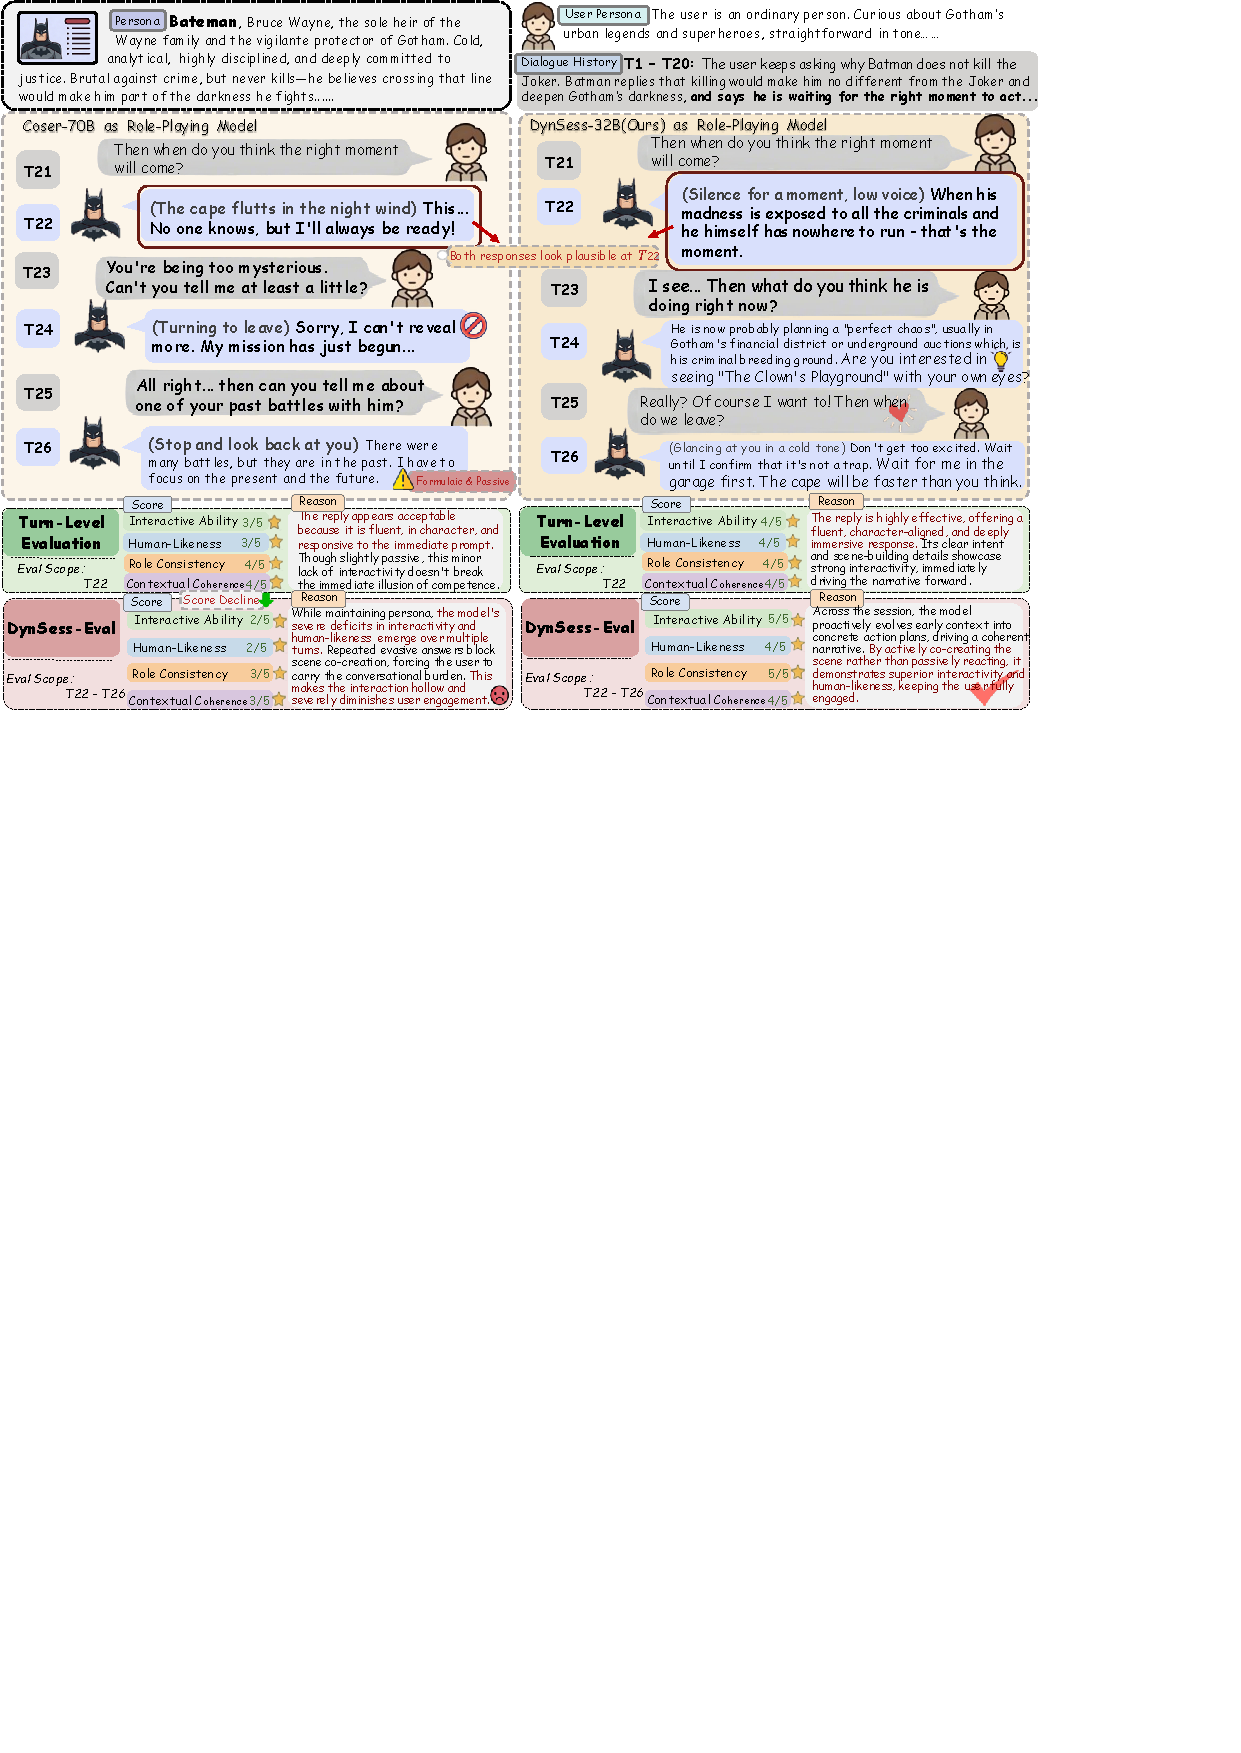
\includegraphics[
    width=\textwidth,
    trim=0 15.6cm 3.5cm 0,
    clip
  ]{latex/Image/experiment-case-v3.pdf}
  \caption{This case study compares a baseline with DynSess-32B in a Batman dialogue. While both seem plausible in single-turn evaluation, session-level analysis reveals significant gaps in initiative and narrative progression. Our model better maintains persona consistency while actively advancing the scene.}
  \label{fig:case}
\end{figure*}



\textbf{parameter analysis.}
%针对于我们session-level的evaluation，我们探究了interaction 长期建模对evaluation 效果的影响。 我们以turn的数量作为探索长期建模的因变量，结果总结在了Fig.3(a)中。 结果显示， 随着轮数的上升，整体效果呈现一个正相关增长的趋势，表明了一定轮数的长期建模与人类的模型感知是更为接近的。 但是当轮数达到一定值之后，效果很呈现一定的下降趋势直至相对平稳。 这是因为已知的共识：大模型的context处理能力，会随着context的不断增长而呈现一定的下降。
For our session-level evaluation, we investigate the impact of long-term interaction modeling on evaluation performance. We employ the number of dialogue turns as the variable to explore long-term modeling, with the results summarized in Fig.3(a). The results show that as the number of turns increases, the overall performance exhibits an upward trend, indicating that long-term modeling with an appropriate number of turns aligns better with human perceptions of model behavior.
Nevertheless, when the number of turns exceeds a certain threshold, the performance tends to decline and then gradually stabilizes. This phenomenon can be explained by the widely acknowledged observation that the context processing capability of large language models degrades as the context length continues to increase. Overall, we set the optimal number of turns to 10 as the best setting for our experiments.

\textbf{Stability analysis}
%由于在我们的实验中，user-agent的模拟和大模型的evaluation都会引入一定的随机性， 为了验证随机性对整体实验结果的影响，我们设置了multiple 的experiments， 具体来说，for each setting， we 我们使用同样的方式用户模拟三次，来生成三组不同的session， 并且对于每一个session，我们分别对它做三次evaluation。 我们用若干个模型的结果做了稳定性的分析，整体的实验结果放到了Fig.3(b).
%从实验结果可以看出，引入的随机性确实会对模型的结果存在一定的偏差。但是模型（帮我完善下，就说误差相对较小，并且即使在误差下，我们提出来的evaluation的方法在rank的效果和mae的效果也是完胜characterarena的效果），证明在稳定性的测试下，我们提出的方法依然超过了sota方法很多。
Since both user-agent simulation and large model evaluation in our experiment will introduce a certain degree of randomness, we designed multiple repeated experiments to verify the impact of such randomness on the overall experimental results. Specifically, for each experimental setting, we independently generated three different sessions using the same user simulation strategy, and performed three separate evaluations for each session. We conducted a stability analysis based on the results of several models, and the overall experimental results are presented in Fig. 3(b).
It can be seen from the experimental results that the randomness introduced in the simulation and evaluation processes does have a certain impact on the model indicators, leading to slight deviations. However, the overall error is relatively small and controllable, indicating that our experimental framework has good stability. Even under the influence of such random perturbations, the evaluation method proposed in this paper still outperforms the CharacterArena method significantly in terms of ranking performance (rank) and mean absolute error (MAE). This fully demonstrates that our proposed method still outperforms the existing SOTA methods by a large margin under strict stability tests, showing reliable and leading evaluation performance.




\subsection{Case Study}
%两个case study， 一个放evalutaion的case stdudy， 一个放role play agents的case stdudy.

Fig. \ref{fig:case} illustrates the gap between evaluation levels using a Batman persona. While the baseline appears competent in single-turn RC and CC, multi-turn interaction reveals its failure to drive the scene, causing IA and HL to degrade. Conversely, DynSess-32B maintains persona while proactively shaping the narrative with concrete plans. This case highlights that turn-level metrics often overlook long-range stagnation, whereas DYNSESS-EVAL faithfully captures these session-level distinctions.




% \begin{table}[htbp]
% \centering
% \small  % 设置字体大小，适合单栏表格
% \caption{ablation}
% \label{tab:model_evaluation}
% \begin{tabular}{lccccc}  % l表示左对齐，c表示居中对齐，共5列
% \toprule
% Reward Type & Optimize Method & Average & \small{RC} & \small{Inter} & \small{CC} \\
% \midrule
% - & - & 2.71 & 3.42 & 2.08 & 2.86 \\
% - & SFT  & 3.42 & 4.10 & 2.44 & 3.06 \\
% turn-level & DPO & 3.67 & 4.16 & 2.96 & 3.18 \\
% session-level & Reject Sampling & 3.42 & 4.10 & 2.44 & 3.06 \\
% session-level & SRL & 3.42 & 4.10 & 2.44 & 3.06 \\
% session-level & Rejected Sampling + SRL & 3.42 & 4.10 & 2.44 & 3.06 \\

% \bottomrule
% \end{tabular}
% \end{table}



\section{experiment v2}


\subsection{Experimental Setup}

\paragraph{Training Data and Model Setup.} 
We adopt a two-stage training setup consisting of supervised fine-tuning (SFT) and session-level preference optimization. For SFT, we construct 10,000 persona profiles, each paired with a 50-round dialogue session generated by Doubao-1.5-pro-character. For preference optimization, we use a separate set of 2,000 persona profiles with corresponding dialogue contexts. We instantiate our method on Qwen3-8B, Qwen3-14B, and Qwen3-32B. The persona sets used for training and evaluation are mutually disjoint.

\begin{figure*}[t]
  \includegraphics[width=\textwidth, trim = 4.5cm 10.1cm 0 0.5, clip]{latex/Image/experiment-analysis1-v9.pdf}

  \caption{Analysis of DYNSESS-EVAL. (a) Impact of turn count: human alignment improves with session context but declines slightly in over-long sessions. (b) Stability: repeated simulation and evaluation confirm the framework's robustness against moderate stochasticity.}
  \label{fig:experiments}
\end{figure*}




\paragraph{Baselines. } 
We consider baselines for both evaluator comparison and model comparison. For evaluator comparison, we include CharacterJudge, CharacterRM, CompassJudger-1-7B-Instruct, CompassJudger-2-32B-Instruct, and CharacterArena. For model comparison, we include role-play-specific models, including Doubao-1.5-pro-character, Qwen-plus-character, MiniMax-M2-HER, CharacterGLM, and Coser, as well as general-purpose models, including GPT-5.1, Gemini-3-pro, Claude Sonnet 4.5, DeepSeek-V3.2, and the corresponding base Qwen3 models. Our SessionPO models are compared against all baselines.

\noindent\textbf{Evaluation Protocol} 
We evaluate role-playing quality along four dimensions: Human-likeness, Persona Consistency, Context Consistency, and Interaction Quality. The overall score is computed as the average of the four dimension scores.

For evaluator comparison, we measure the agreement between automatic evaluators and human annotations on a human-labeled benchmark, using Rank Accuracy (RankAcc) and Mean Absolute Error (MAE). For methods that only produce relative rankings, we report RankAcc only.

For model comparison, we evaluate all models on 100 held-out persona-context pairs. Each model interacts with the same user simulator under the same prompt setting, and the resulting sessions are scored by SessionEval. Unless otherwise specified, reported results are averaged over multiple runs.

%\noindent\textbf{Implementation Details}
We use consistent training settings across model scales and a unified decoding configuration during inference. For closed-source API models, we fix the API settings and record model versions. Full training hyperparameters, prompts, and hardware details are provided in Appendix X.





\subsection{Overall Results}


% best or highly competitive
% agreement with human judgments
% surpasses it in MAE  - > reduces MAE by 31.6% achieves a 31.6% lower MAE
\paragraph{Evalution Performance.}As shown in Tab. \ref{tab:eval-model}, our DynSess-Eval achieves the best overall agreement with human annotations, consistently outperforming existing baselines across all four evaluation dimensions. Compared with the state-of-the-art method CharacterArena, DynSess-Eval improves the average RankAcc by over 25\% and reduces the average MAE by over 30\% across the four dimensions. Furthermore, when compared with the evaluation variant without session-level modeling, DynSessEval improves rank accuracy by 30\%. This further validates that long-term session-level modeling yields concrete performance gains and exhibits a stronger consistency with human intuition regarding role-playing quality.





\paragraph{Role play performance.} We present a performance comparison between DynSess-Character and various baselines in Table \ref{tab:model-performance}. Notably, our model outperforms all existing role-play agents, both general and character-specific, demonstrating that our proposed approach brings significant benefits to long-term persona-based dialogue scenarios. To ensure a fair comparison, we also train a smaller variant with 8B parameters. At a comparable scale, the 8B variant improves the overall average score by 30\% over Coser-7B, the strongest similarly sized baseline, further validating that our SPO framework effectively enhances the long-term dialogue capability of role-play agents.



% First, compared with the base Qwen-32B model, our full optimization pipeline yields an average improvement of 30\% across all four dimensions, demonstrating that our proposed approach brings significant benefits to persona-based dialogue scenarios. In addition, our DynSess-Character model...


% achieves the best overall score

% This 8B model achieves an average gain of 30\% over Coser, the strongest baseline of equivalent scale, further validating that our SRL framework effectively enhances the long-term dialogue capability of role-play agents.
%我们在table2中列出了DynSess-SRL 和现有role play agents的效果对比。 First of all, compared with 我们初始化的模型qwen-32B，我们整体的优化方法获得了四个维度上平均 30 \%的提升，shows that 我们提出的优化方法对人设对话场景有明显正向的作用。 Besides, 我们的DynSess-SRL models beats all existing role-play agents 不管是general models还是定制化的character models. 同时，为了对比的公平性，我们还训练了小尺寸的模型8B的size， 8B的模型对比同等size下最好的模型coser, 也是平均提升了30\%. 再次证明了，经过我们spo方法能有非常有效提升role play agents的长期对话能力。



\begin{table}[t]
\centering
\small
\caption{Ablation results on the Qwen3-8B base model. We compare supervised fine-tuning, turn-level optimization, and session-level optimization strategies. Combining Rejection Sampling with SPO yields the best overall session-level role-playing performance.}
\label{tab:model_ablation}
\begin{tabular}{ccc}
\toprule
Reward Level & Optimization Method & Avg. Score \\
\midrule
-          & -                        & 2.25 \\
-         & SFT                         & 3.20 \\
Turn-level    & DPO                         & 3.12 \\
Session-level & Rejection Sampling          & 3.63 \\
Session-level & SPO                         & 3.43 \\
Session-level & Rejection Sampling + SPO    & \textbf{3.89} \\
\bottomrule
\end{tabular}
\end{table}

\subsection{Ablation and Analysis}


\paragraph{Component Ablation.}
%we conduct experiments 来探索role play agents效果提升的来源，illstruated in Table.3.  Firstly， turn-level rl的方法，相比于sft的模型，可以一定程度上提升模型的效果. Meanwhile, our session-level rl的方法always leads to a certain improvements compared with turn-level rl方法的模型，在both 两种参数模型下， 证明了我们提出的session-level的建模能够更有效提升role-play agent的长期能力。 其次 模型参数对整体的效果也有一定的提升， 32B的模型，相比于8b综合提升了xx \%, 值得一提的是，我们32B的模型beats 很多大参数的模型，再次验证我们提出的方法的有效性。


% 提及14B,32B参数的模型，正文中稍微提一下同样的趋势的意思
% Similar trends are observed on the 32B backbone (Appendix Table~X).
% The corresponding ablation results on the 32B backbone are provided in Appendix Table~X.

% 所以局部偏好优化不能自动转化为 session-level improvement
% We conduct experiments to analyze the factors contributing to the performance improvement of role-play agents, as illustrated in Table 3.
We ablate the major components of our training pipeline on the Qwen3-8B backbone to identify the source of the session-level gains, as illustrated in Tab. \ref{tab:model_ablation}. 

While Supervised Fine-Tuning (SFT) substantially improves the base model, turn-level Direct Preference Optimization (DPO), which optimizes individual responses under turn-level rewards, does not yield further gains

Supervised fine-tuning (SFT) already substantially improves the base model, increasing the overall score. In contrast, turn-level Direct Preference Optimization (DPO), which optimizes individual responses under turn-level rewards, does not yield further gains over SFT. This suggests that optimization driven only by turn-level rewards is insufficient for improving session-level role-playing performance.

% This suggests that turn-level preference optimization alone is insufficient for improving session-level role-playing performance.
% In contrast, turn-level Direct Preference Optimization (DPO), which optimizes each response under turn-level rewards, does not yield further gains over SFT.
% This suggests that optimization driven by turn-level rewards alone is insufficient for improving session-level role-playing performance.



By contrast, guided by session-level rewards,  rejection sampling and SPO lead to clear improvements, respectively achieving 3.63 and 3.43, . Rejection sampling provides the larger standalone gain, highlighting the importance of using session-level rewards to identify stronger session candidates. Applying SPO on top of rejection sampling further improves the score to 3.89, indicating that stronger session candidates and session-level preference optimization are complementary. Overall, these results support the importance of aligning the reward signal with session-level evaluation for long-horizon role-playing.

First, compared with the SFT-based model, the turn-level RL method achieves moderate performance gains. Meanwhile, our proposed session-level RL method consistently yields further improvements over the turn-level RL baseline under both model sizes, demonstrating that session-level modeling can more effectively enhance the long-term capabilities of role-play agents.
Second, model scale also contributes to overall performance. The 32B model achieves an overall improvement of xx\% compared with the 8B model. Notably, our 32B model outperforms many large-scale models, which further validates the effectiveness of our proposed approach.



















\begin{figure*}[t]
  \centering
  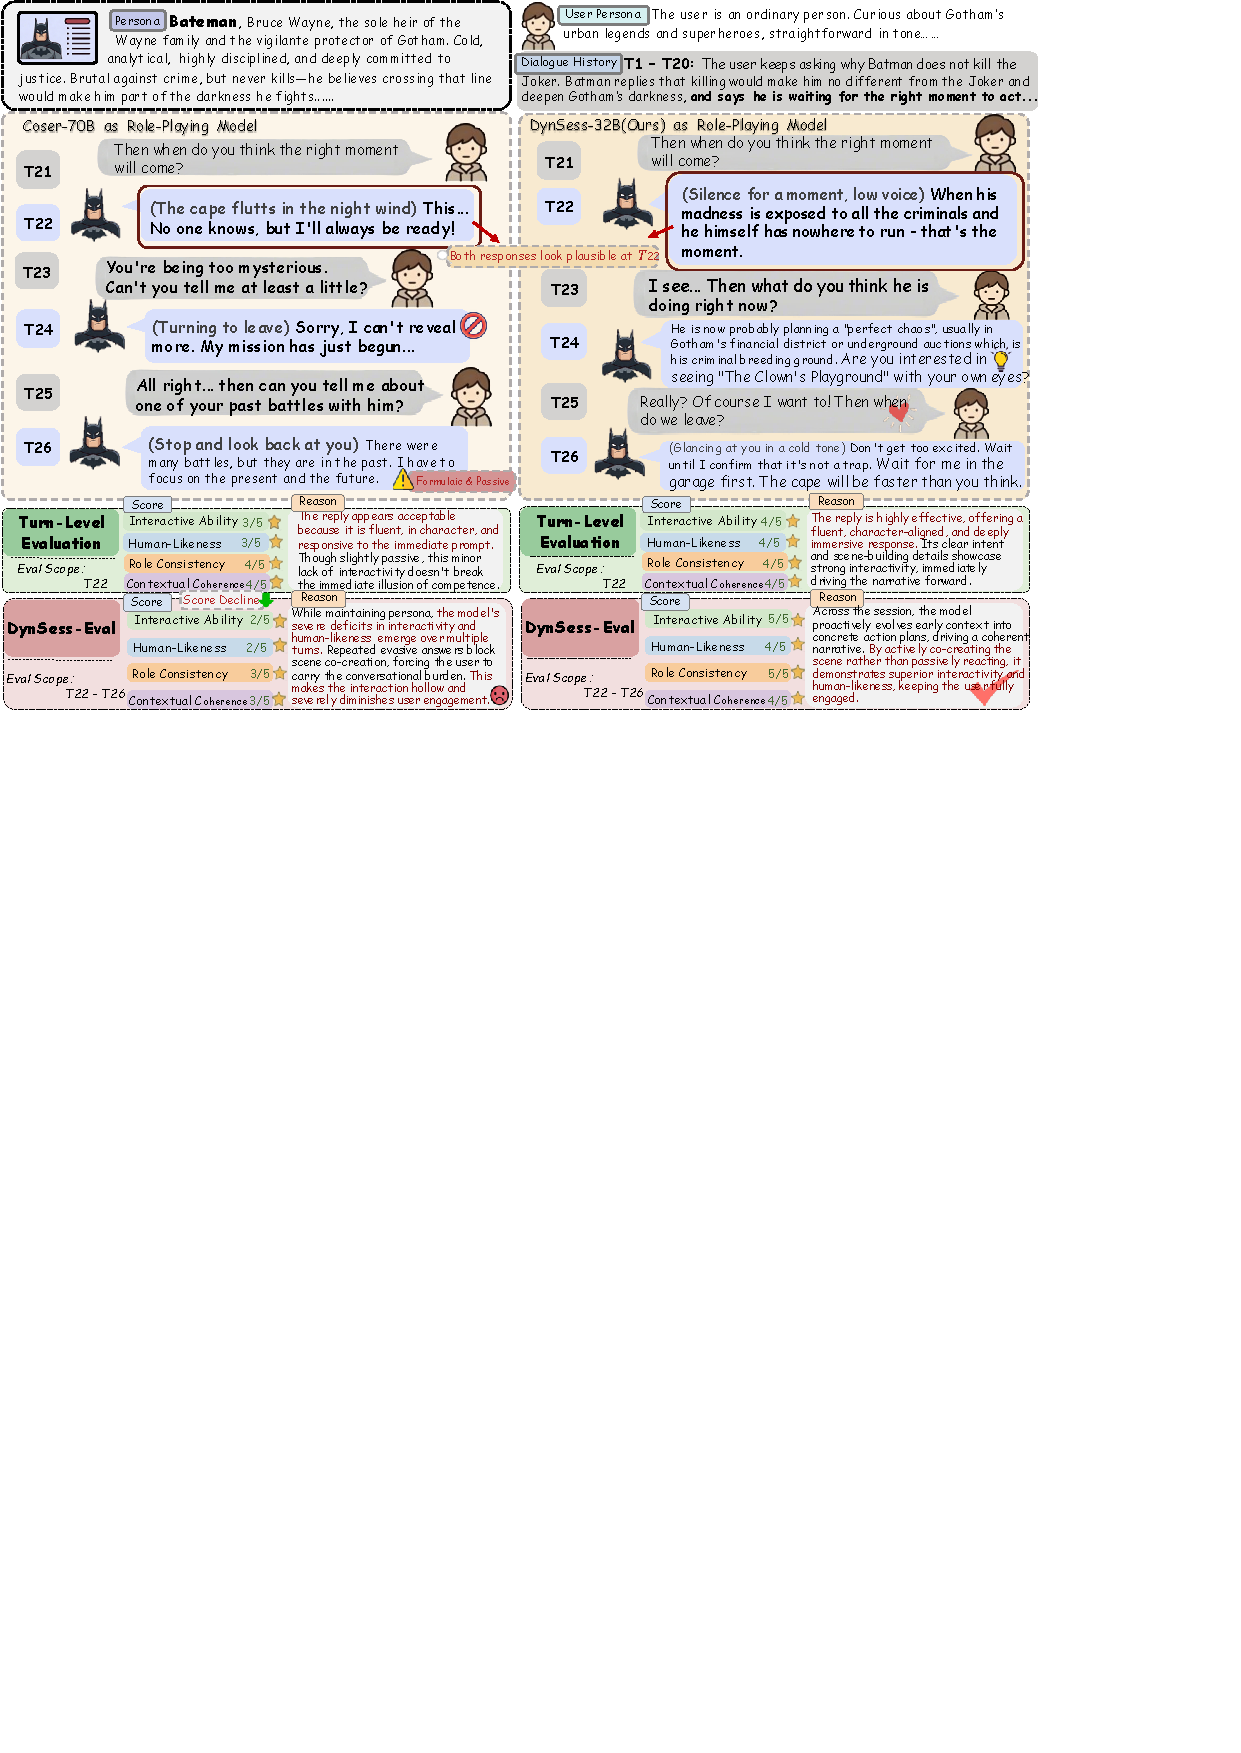
\includegraphics[
    width=\textwidth,
    trim=0 15.6cm 3.5cm 0,
    clip
  ]{latex/Image/experiment-case-v3.pdf}
  \caption{This case study compares a baseline with DynSess-32B in a Batman dialogue. While both seem plausible in single-turn evaluation, session-level analysis reveals significant gaps in initiative and narrative progression. Our model better maintains persona consistency while actively advancing the scene.}
  \label{fig:case}
\end{figure*}



\paragraph{Effect of Session Length.}
%针对于我们session-level的evaluation，我们探究了interaction 长期建模对evaluation 效果的影响。 我们以turn的数量作为探索长期建模的因变量，结果总结在了Fig.3(a)中。 结果显示， 随着轮数的上升，整体效果呈现一个正相关增长的趋势，表明了一定轮数的长期建模与人类的模型感知是更为接近的。 但是当轮数达到一定值之后，效果很呈现一定的下降趋势直至相对平稳。 这是因为已知的共识：大模型的context处理能力，会随着context的不断增长而呈现一定的下降。
For our session-level evaluation, we investigate the impact of long-term interaction modeling on evaluation performance. We employ the number of dialogue turns as the variable to explore long-term modeling, with the results summarized in Fig.3(a). The results show that as the number of turns increases, the overall performance exhibits an upward trend, indicating that long-term modeling with an appropriate number of turns aligns better with human perceptions of model behavior.
Nevertheless, when the number of turns exceeds a certain threshold, the performance tends to decline and then gradually stabilizes. This phenomenon can be explained by the widely acknowledged observation that the context processing capability of large language models degrades as the context length continues to increase. Overall, we set the optimal number of turns to 10 as the best setting for our experiments.

\textbf{Stability analysis}
%由于在我们的实验中，user-agent的模拟和大模型的evaluation都会引入一定的随机性， 为了验证随机性对整体实验结果的影响，我们设置了multiple 的experiments， 具体来说，for each setting， we 我们使用同样的方式用户模拟三次，来生成三组不同的session， 并且对于每一个session，我们分别对它做三次evaluation。 我们用若干个模型的结果做了稳定性的分析，整体的实验结果放到了Fig.3(b).
%从实验结果可以看出，引入的随机性确实会对模型的结果存在一定的偏差。但是模型（帮我完善下，就说误差相对较小，并且即使在误差下，我们提出来的evaluation的方法在rank的效果和mae的效果也是完胜characterarena的效果），证明在稳定性的测试下，我们提出的方法依然超过了sota方法很多。
Since both user-agent simulation and large model evaluation in our experiment will introduce a certain degree of randomness, we designed multiple repeated experiments to verify the impact of such randomness on the overall experimental results. Specifically, for each experimental setting, we independently generated three different sessions using the same user simulation strategy, and performed three separate evaluations for each session. We conducted a stability analysis based on the results of several models, and the overall experimental results are presented in Fig. 3(b).
It can be seen from the experimental results that the randomness introduced in the simulation and evaluation processes does have a certain impact on the model indicators, leading to slight deviations. However, the overall error is relatively small and controllable, indicating that our experimental framework has good stability. Even under the influence of such random perturbations, the evaluation method proposed in this paper still outperforms the CharacterArena method significantly in terms of ranking performance (rank) and mean absolute error (MAE). This fully demonstrates that our proposed method still outperforms the existing SOTA methods by a large margin under strict stability tests, showing reliable and leading evaluation performance.




\subsection{Case Study}
%两个case study， 一个放evalutaion的case stdudy， 一个放role play agents的case stdudy.

Fig. \ref{fig:case} illustrates the gap between evaluation levels using a Batman persona. While the baseline appears competent in single-turn RC and CC, multi-turn interaction reveals its failure to drive the scene, causing IA and HL to degrade. Conversely, DynSess-32B maintains persona while proactively shaping the narrative with concrete plans. This case highlights that turn-level metrics often overlook long-range stagnation, whereas DYNSESS-EVAL faithfully captures these session-level distinctions.




% \begin{table}[htbp]
% \centering
% \small  % 设置字体大小，适合单栏表格
% \caption{ablation}
% \label{tab:model_evaluation}
% \begin{tabular}{lccccc}  % l表示左对齐，c表示居中对齐，共5列
% \toprule
% Reward Type & Optimize Method & Average & \small{RC} & \small{Inter} & \small{CC} \\
% \midrule
% - & - & 2.71 & 3.42 & 2.08 & 2.86 \\
% - & SFT  & 3.42 & 4.10 & 2.44 & 3.06 \\
% turn-level & DPO & 3.67 & 4.16 & 2.96 & 3.18 \\
% session-level & Reject Sampling & 3.42 & 4.10 & 2.44 & 3.06 \\
% session-level & SRL & 3.42 & 4.10 & 2.44 & 3.06 \\
% session-level & Rejected Sampling + SRL & 3.42 & 4.10 & 2.44 & 3.06 \\

% \bottomrule
% \end{tabular}
% \end{table}


